\documentclass[aspectratio=169]{beamer}
\usetheme{default}
\setbeamertemplate{navigation symbols}{}
\setbeamertemplate{footline}{}
\usepackage{tikz}
\usetikzlibrary{positioning,arrows.meta,shapes,shapes.multipart,
                shapes.geometric,shapes.misc,fit,backgrounds,calc}
\usepackage{xcolor}

\definecolor{hdrblue}{RGB}{25,70,145}
\definecolor{hdrbg}{RGB}{205,220,250}
\definecolor{clsbg}{RGB}{238,245,255}
\definecolor{abstrhdr}{RGB}{140,85,0}
\definecolor{abstrbg}{RGB}{255,243,215}
\definecolor{lgray}{RGB}{90,110,150}

\definecolor{sysblue}{RGB}{20,70,140}
\definecolor{sysfill}{RGB}{228,237,255}
\definecolor{ucbdr}{RGB}{50,110,200}
\definecolor{ucfill}{RGB}{248,252,255}
\definecolor{extbdr}{RGB}{155,95,0}
\definecolor{extfill}{RGB}{255,246,210}
\definecolor{actbdr}{RGB}{30,90,160}
\definecolor{actfill}{RGB}{235,245,255}

\definecolor{procblue}{RGB}{25,75,150}
\definecolor{procfill}{RGB}{210,228,255}
\definecolor{stgreen}{RGB}{0,110,60}
\definecolor{stfill}{RGB}{210,245,225}
\definecolor{extbrn}{RGB}{135,65,0}
\definecolor{extfillb}{RGB}{255,240,210}
\definecolor{arrgray}{RGB}{80,100,130}

\definecolor{navy}{RGB}{15,55,130}
\definecolor{steelblue}{RGB}{50,100,180}
\definecolor{skyblue}{RGB}{200,220,255}
\definecolor{teal}{RGB}{0,120,110}
\definecolor{tealfill}{RGB}{200,240,235}
\definecolor{amber}{RGB}{155,85,0}
\definecolor{amberfill}{RGB}{255,235,195}
\definecolor{violet}{RGB}{100,30,150}
\definecolor{violetfill}{RGB}{235,215,255}
\definecolor{layerbg}{RGB}{245,248,255}
\definecolor{layerbdr}{RGB}{150,175,225}
\definecolor{arrcol}{RGB}{60,80,120}
\definecolor{red2}{RGB}{175,30,30}
\definecolor{redfill}{RGB}{255,215,215}

\begin{document}

% =============================================================
% FRAME 1: CLASS DIAGRAM
% =============================================================
\begin{frame}[plain]
\vspace{-0.25cm}
\begin{center}{\small\bfseries\sffamily\color{hdrblue}
  Class Diagram --- Metamorphic Circuit Breaker Framework}\end{center}
\vspace{-0.15cm}
\centering\resizebox{!}{0.82\textheight}{%
\begin{tikzpicture}[font=\tiny\sffamily]
\tikzset{
  CB/.style={draw=hdrblue,thick,rectangle split,rectangle split parts=3,
    rectangle split part fill={hdrbg,clsbg,clsbg},
    text width=2.4cm,align=left,inner sep=2.5pt,rounded corners=1pt},
  AB/.style={draw=abstrhdr,thick,rectangle split,rectangle split parts=3,
    rectangle split part fill={abstrbg,white,white},
    text width=2.4cm,align=left,inner sep=2.5pt,rounded corners=1pt},
  assoc/.style={->,>=Latex,thick,lgray},
  compose/.style={-{Diamond[open]},thick,hdrblue},
  inherit/.style={-{Triangle[open]},thick,abstrhdr},
  dep/.style={->,>=Latex,dashed,thick,gray},
}

\node[CB](img) at (0,0){
  \textbf{\color{hdrblue}InputImage}\nodepart{two}
  \texttt{- imageId : String}\\
  \texttt{- rawData : Tensor}\\
  \texttt{- source : String}\nodepart{three}
  \texttt{+ load() : Tensor}\\
  \texttt{+ resize(w,h) : Tensor}};

\node[CB](te) at (4,0){
  \textbf{\color{hdrblue}TransformationEngine}\nodepart{two}
  \texttt{- transforms : List}\\
  \texttt{- calibData : Dataset}\nodepart{three}
  \texttt{+ calibrate() : void}\\
  \texttt{+ apply(img) : List}};

\node[AB](tr) at (8,0){
  \textit{\color{abstrhdr}$\langle\langle$\rangle\rangle$ Transform}\nodepart{two}
  \texttt{- name : String}\\
  \texttt{- severity : float}\nodepart{three}
  \texttt{+ apply(img) : Tensor}\\
  \texttt{+ validate() : bool}};

\node[CB](sc) at (12,0){
  \textbf{\color{hdrblue}StabilityChecker}\nodepart{two}
  \texttt{- threshold : float}\\
  \texttt{- windowSize : int}\nodepart{three}
  \texttt{+ check() : bool}\\
  \texttt{+ computeDisag() : float}};

\node[CB](rot) at (4.5,-2.8){
  \textbf{\color{hdrblue}RotationTransform}\nodepart{two}
  \texttt{- angle : float}\nodepart{three}
  \texttt{+ apply() : Tensor}};

\node[CB](bri) at (7.0,-2.8){
  \textbf{\color{hdrblue}BrightnessTransform}\nodepart{two}
  \texttt{- factor : float}\nodepart{three}
  \texttt{+ apply() : Tensor}};

\node[CB](crp) at (9.5,-2.8){
  \textbf{\color{hdrblue}CropTransform}\nodepart{two}
  \texttt{- ratio : float}\nodepart{three}
  \texttt{+ apply() : Tensor}};

\node[CB](noi) at (12.0,-2.8){
  \textbf{\color{hdrblue}NoiseTransform}\nodepart{two}
  \texttt{- stdDev : float}\nodepart{three}
  \texttt{+ apply() : Tensor}};

\node[AB](vm) at (0,-5.5){
  \textit{\color{abstrhdr}$\langle\langle$\rangle\rangle$ VisionModel}\nodepart{two}
  \texttt{- modelId : String}\\
  \texttt{- version : String}\nodepart{three}
  \texttt{+ predict() : Prediction}\\
  \texttt{+ batchPredict() : List}};

\node[CB](pred) at (4,-5.5){
  \textbf{\color{hdrblue}Prediction}\nodepart{two}
  \texttt{- label : String}\\
  \texttt{- confidence : float}\nodepart{three}
  \texttt{+ isReliable() : bool}\\
  \texttt{+ getLabel() : String}};

\node[CB](cb) at (8,-5.5){
  \textbf{\color{hdrblue}CircuitBreaker}\nodepart{two}
  \texttt{- state : CBState}\\
  \texttt{- failureCount : int}\nodepart{three}
  \texttt{+ evaluate() : Action}\\
  \texttt{+ trip() : void}};

\node[AB](cbs) at (12,-5.5){
  \textit{\color{abstrhdr}$\langle\langle$\rangle\rangle$ CBState}\nodepart{two}
  \texttt{CLOSED}\\
  \texttt{OPEN}\\
  \texttt{HALF\_OPEN}\nodepart{three}\phantom{x}};

\node[CB](fh) at (0,-9.0){
  \textbf{\color{hdrblue}FallbackHandler}\nodepart{two}
  \texttt{- strategy : String}\nodepart{three}
  \texttt{+ handle() : Prediction}\\
  \texttt{+ routeToHuman() : void}};

\node[CB](ood) at (4,-9.0){
  \textbf{\color{hdrblue}OODDataset}\nodepart{two}
  \texttt{- samples : List}\nodepart{three}
  \texttt{+ generate() : void}\\
  \texttt{+ getSample() : Tensor}};

\node[CB](me) at (8,-9.0){
  \textbf{\color{hdrblue}MetricsEvaluator}\nodepart{two}
  \texttt{- auroc : float}\nodepart{three}
  \texttt{+ computeAUROC() : float}\\
  \texttt{+ reportOverhead() : float}};

\node[CB](ot) at (12,-9.0){
  \textbf{\color{hdrblue}OfflineTester}\nodepart{two}
  \texttt{- testDataset : OODDataset}\nodepart{three}
  \texttt{+ runTest() : Report}\\
  \texttt{+ detectWeaknesses() : List}};

\draw[assoc]   (img.east) -- node[above,font=\tiny\sffamily]{uses} (te.west);
\draw[compose] (te.east)  -- node[above,font=\tiny\sffamily]{contains} (tr.west);
\draw[assoc]   (tr.east)  -- node[above,font=\tiny\sffamily]{feeds} (sc.west);

\draw[inherit] (rot.north) -- ++(0,0.55) -| (tr.south);
\draw[inherit] (bri.north) -- ++(0,0.55) -| (tr.south);
\draw[inherit] (crp.north) -- ++(0,0.55) -| (tr.south);
\draw[inherit] (noi.north) -- ++(0,0.55) -| (tr.south);

\draw[assoc] (img.south) -- (vm.north);
\draw[assoc] (vm.east)   -- node[above,font=\tiny\sffamily]{produces} (pred.west);
\draw[assoc] (pred.east) -- node[above,font=\tiny\sffamily]{evaluated by} (cb.west);
\draw[assoc] (cb.east)   -- node[above,font=\tiny\sffamily]{state} (cbs.west);

\draw[assoc] (sc.south) -- ++(0,-0.9) -- ++(1.8,0) -- ++(0,-2.2) -- ++(-5.8,0) -- (cb.north);
\draw[assoc] (cb.south) -- ++(0,-0.9) -- ++(-8.0,0) -- (fh.north);
\draw[dep] (fh.west) -- ++(-0.7,0) -- ++(0,3.5) -- (vm.west);

\draw[dep]   (fh.east)  -- node[above,font=\tiny\sffamily]{uses} (ood.west);
\draw[assoc] (ood.east) -- node[above,font=\tiny\sffamily]{evaluated by} (me.west);
\draw[assoc] (me.east)  -- node[above,font=\tiny\sffamily]{used in} (ot.west);
\draw[assoc] (ot.south) -- ++(0,-0.6) -- ++(-8.0,0) -- (ood.south);

\end{tikzpicture}%
}
\vspace{0.05cm}
{\tiny\sffamily
\tikz[baseline=-0.5ex]{
  \draw[->,>=Latex,thick,lgray](0,0)--(1,0) node[right]{Assoc.\,};
  \draw[-{Diamond[open]},thick,hdrblue](3.5,0)--(4.5,0) node[right]{Composition\,};
  \draw[-{Triangle[open]},thick,abstrhdr](8,0)--(9,0) node[right]{Inheritance\,};
  \draw[->,>=Latex,dashed,thick,gray](12.5,0)--(13.5,0) node[right]{Dependency};
}}
\end{frame}

% =============================================================
% FRAME 2: USE CASE DIAGRAM
% =============================================================
\begin{frame}[plain]
\vspace{-0.25cm}
\begin{center}{\small\bfseries\sffamily\color{sysblue}
  Use Case Diagram --- Metamorphic Circuit Breaker Framework}\end{center}
\vspace{-0.15cm}
\centering\resizebox{!}{0.82\textheight}{%
\begin{tikzpicture}[font=\scriptsize\sffamily]
\tikzset{
  UC/.style={draw=ucbdr,fill=ucfill,thick,ellipse,minimum width=3.6cm,minimum height=1.0cm,font=\scriptsize\sffamily,align=center,inner sep=1pt},
  EC/.style={draw=extbdr,fill=extfill,thick,ellipse,minimum width=3.6cm,minimum height=1.0cm,font=\scriptsize\sffamily,align=center,inner sep=1pt},
  AL/.style={thick,actbdr},
  IA/.style={->,>=Latex,dashed,ucbdr,thick},
  EA/.style={->,>=Latex,dashed,extbdr,thick},
}
\newcommand{\ACT}[3]{%
  \begin{scope}[shift={(#1,#2)}]
    \draw[thick,actbdr,fill=actfill](0,0.46)circle(0.19cm);
    \draw[thick,actbdr](0,0.27)--(0,-0.10);
    \draw[thick,actbdr](-0.23,0.08)--(0.23,0.08);
    \draw[thick,actbdr](0,-0.10)--(-0.18,-0.42);
    \draw[thick,actbdr](0,-0.10)--(0.18,-0.42);
    \node[font=\scriptsize\bfseries\sffamily,text=actbdr,align=center,below=0.48cm] at (0,0){#3};
  \end{scope}}

\draw[draw=sysblue,fill=sysfill,thick,rounded corners=7pt] (1.0,6.0) rectangle (15.5,-5.2);
\node[font=\small\bfseries\sffamily\color{sysblue},anchor=north west] at (1.2,6.0){Metamorphic Circuit Breaker System};

\ACT{-1.0}{4.0}{ML Engineer}
\ACT{-1.0}{0.5}{Vision Model}
\ACT{-1.0}{-3.0}{Deployment\\[-1pt]Env.}

\ACT{16.8}{3.2}{Human\\[-1pt]Reviewer}
\ACT{16.8}{0.5}{Fallback\\[-1pt]Model}
\ACT{16.8}{-2.5}{Monitoring\\[-1pt]System}

\node[UC](uc1)  at (3.8, 5.0){Calibrate\\Transformations};
\node[UC](uc2)  at (3.8, 3.5){Run Offline\\Metamorphic Test};
\node[UC](uc3)  at (3.8, 2.0){Configure\\Circuit Breaker};
\node[UC](uc4)  at (3.8, 0.5){Submit\\Input Image};
\node[UC](uc5)  at (3.8,-1.0){Trigger Online\\Monitoring};
\node[UC](uc6)  at (3.8,-2.5){Sample / Filter\\Predictions};
\node[UC](uc7)  at (3.8,-4.0){Detect\\Weaknesses};

\node[UC](uc8)  at (8.5, 5.0){Apply Semantic\\Transformations};
\node[UC](uc9)  at (8.5, 3.5){Batch Inference\\on Variants};
\node[UC](uc10) at (8.5, 2.0){Check Prediction\\Stability};
\node[UC](uc11) at (8.5, 0.5){Evaluate\\Consistency};
\node[UC](uc12) at (8.5,-1.0){Trip Circuit\\Breaker};
\node[UC](uc13) at (8.5,-2.5){Reset Circuit\\Breaker};
\node[UC](uc14) at (8.5,-4.0){Generate OOD\\Test Dataset};

\node[EC](uc15) at (13.2, 4.2){Route to\\Human Reviewer};
\node[EC](uc16) at (13.2, 2.7){Route to\\Fallback Model};
\node[EC](uc17) at (13.2, 1.2){Flag as\\Low-Confidence};
\node[UC](uc18) at (13.2,-0.3){Compute AUROC\\/ FPR95};
\node[UC](uc19) at (13.2,-1.8){Report Inference\\Overhead};
\node[UC](uc20) at (13.2,-3.3){Produce\\Reliability Report};

\draw[AL](-0.8,4.0)--(uc1.west);
\draw[AL](-0.8,4.0)--(uc2.west);
\draw[AL](-0.8,4.0)--(uc3.west);
\draw[AL](-0.8,4.0)--(uc7.west);

\draw[AL](-0.8,0.5)--(uc4.west);
\draw[AL](-0.8,0.5)--++(1.5,0)--++(0,3.0)--(uc9.west);

\draw[AL](-0.8,-3.0)--(uc5.west);
\draw[AL](-0.8,-3.0)--(uc6.west);

\draw[AL](16.6,3.2)--(uc15.east);
\draw[AL](16.6,0.5)--(uc16.east);
\draw[AL](16.6,-2.5)--(uc18.east);
\draw[AL](16.6,-2.5)--(uc19.east);
\draw[AL](16.6,-2.5)--(uc20.east);

\draw[IA](uc1.east)--node[above,font=\tiny\sffamily]{$\langle\langle$\rangle\rangle$}(uc8.west);
\draw[IA](uc2.east)--node[above,font=\tiny\sffamily]{$\langle\langle$\rangle\rangle$}(uc9.west);
\draw[IA](uc5.east)--++(0.4,0)--++(0,3.2)--(uc10.west);
\draw[IA](uc8.south)--node[right,font=\tiny\sffamily]{$\langle\langle$\rangle\rangle$}(uc9.north);
\draw[IA](uc10.south)--node[right,font=\tiny\sffamily]{$\langle\langle$\rangle\rangle$}(uc11.north);
\draw[IA](uc11.south)--node[right,font=\tiny\sffamily]{$\langle\langle$\rangle\rangle$}(uc12.north);
\draw[IA](uc7.east)--node[above,font=\tiny\sffamily]{$\langle\langle$\rangle\rangle$}(uc14.west);
\draw[IA](uc2.east)--++(0.5,0)--++(0,-7.9)--(uc14.west);
\draw[IA](uc7.south)--++(0,-0.5)--++(9.4,0)--(uc18.south);
\draw[IA](uc7.east)--++(5.1,0)--++(0,0.7)--(uc20.west);

\draw[EA](uc13.north)--node[right,font=\tiny\sffamily]{\color{extbdr}$\langle\langle$\rangle\rangle$}(uc12.south);
\draw[EA](uc6.north)--node[right,font=\tiny\sffamily]{\color{extbdr}$\langle\langle$\rangle\rangle$}(uc5.south);
\draw[EA](uc19.north)--node[right,font=\tiny\sffamily]{\color{extbdr}$\langle\langle$\rangle\rangle$}(uc18.south);
\draw[EA](uc15.west)--++(-0.5,0)--++(0,-5.5)--(uc12.north east);
\draw[EA](uc16.west)--++(-0.3,0)--++(0,-4.0)--(uc12.east);
\draw[EA](uc17.west)--++(-0.1,0)--++(0,-2.5)--(uc12.south east);

\end{tikzpicture}%
}
\vspace{0.05cm}
{\tiny\sffamily
\tikz[baseline=-0.5ex]{
  \draw[IA](0,0)--(1,0) node[right]{$\langle\langle$\rangle\rangle$\quad};
  \draw[EA](4,0)--(5,0) node[right]{\color{extbdr}$\langle\langle$\rangle\rangle$\quad};
  \draw[AL](8,0)--(9,0) node[right]{Association\quad};
  \draw[EC](12.5,0) ellipse(0.8cm and 0.3cm)
    node[right=0.9cm]{\color{extbdr}External};
}}
\end{frame}

% =============================================================
% FRAME 3: DFD
% =============================================================
\begin{frame}[plain]
\vspace{-0.25cm}
\begin{center}{\small\bfseries\sffamily\color{procblue}
  Data Flow Diagram (Level 1) --- Metamorphic Circuit Breaker Framework}\end{center}
\vspace{-0.15cm}
\centering\resizebox{!}{0.82\textheight}{%
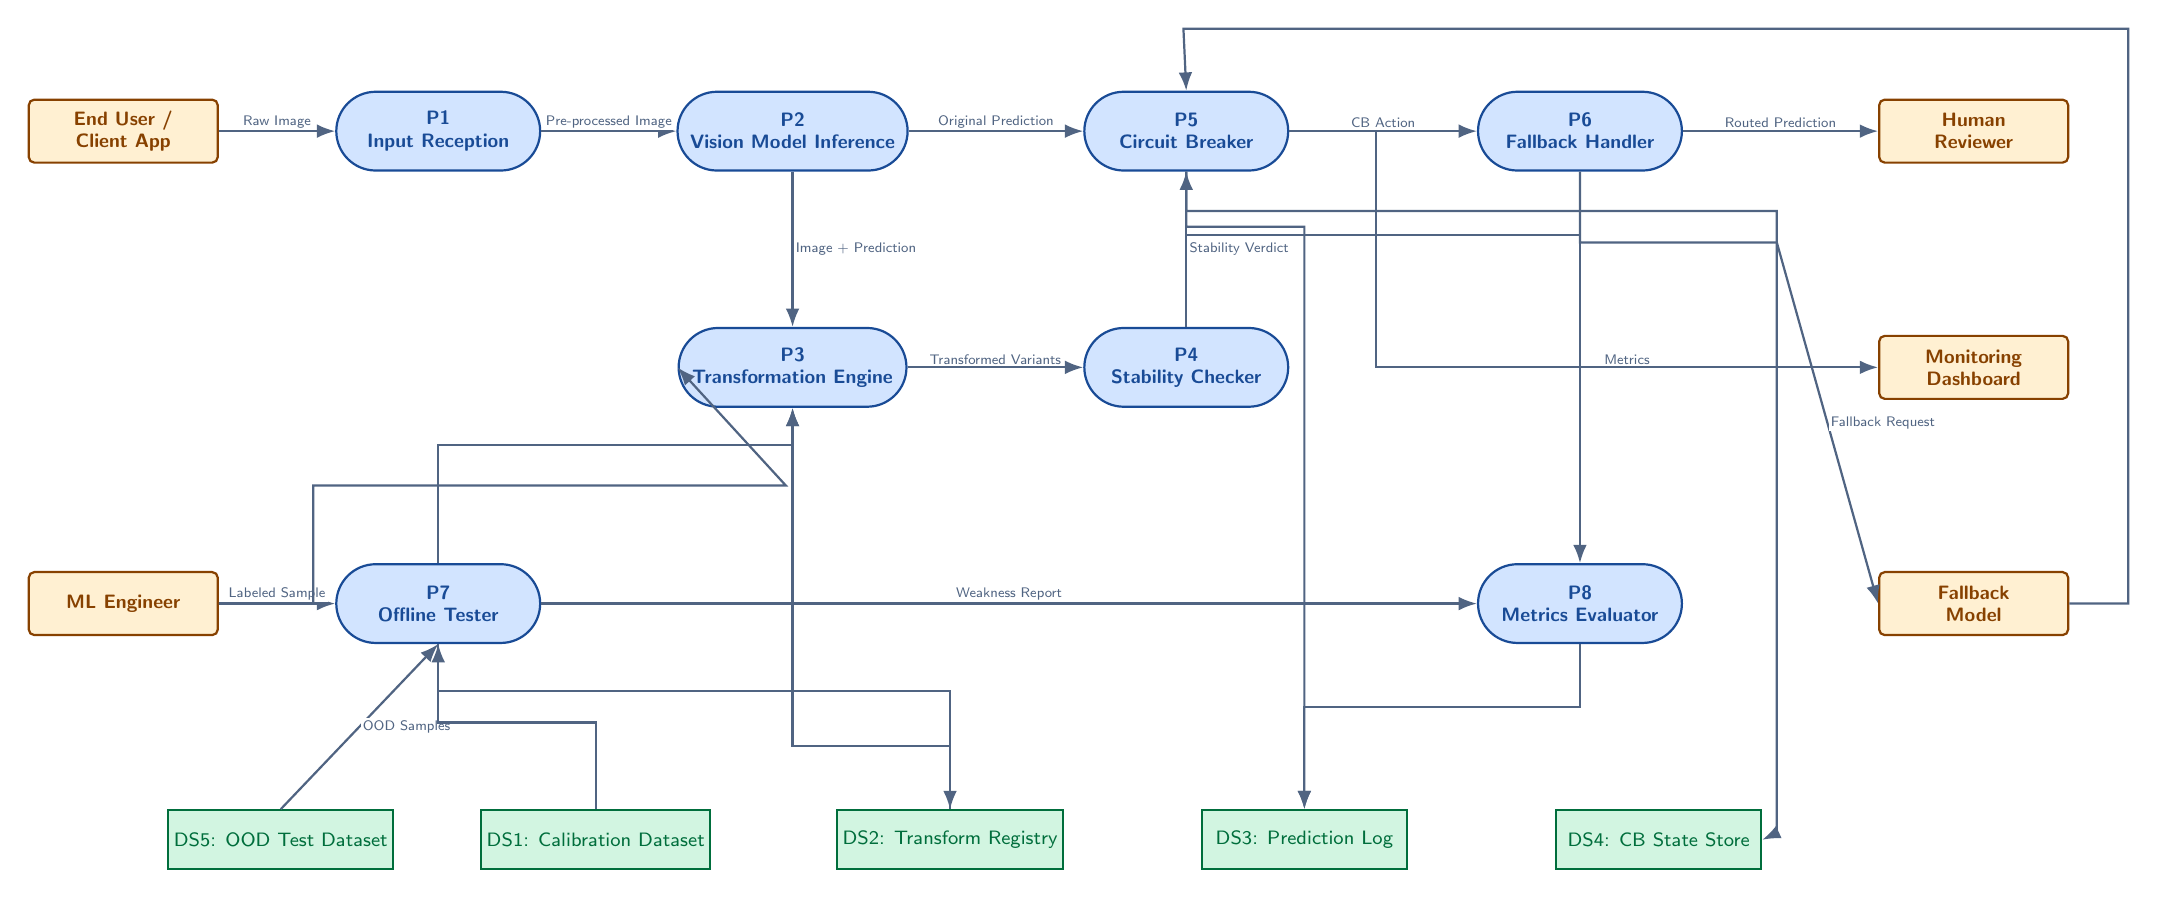
\begin{tikzpicture}[font=\scriptsize\sffamily]
\tikzset{
  PR/.style={draw=procblue,fill=procfill,thick,rounded rectangle,minimum width=2.8cm,minimum height=1.0cm,font=\scriptsize\bfseries\sffamily\color{procblue},align=center,inner sep=3pt},
  DS/.style={draw=stgreen,fill=stfill,thick,rectangle,minimum width=2.6cm,minimum height=0.75cm,font=\scriptsize\sffamily\color{stgreen},align=center,inner sep=2pt},
  EX/.style={draw=extbrn,fill=extfillb,thick,rectangle,minimum width=2.4cm,minimum height=0.8cm,font=\scriptsize\bfseries\sffamily\color{extbrn},align=center,rounded corners=2pt,inner sep=2pt},
  FL/.style={->,>=Latex,thick,arrgray},
  lb/.style={font=\tiny\sffamily,fill=white,inner sep=0.8pt,midway},
}

\node[EX](user)    at ( 0.0, 4.5){End User /\\Client App};
\node[EX](human)   at (23.5, 4.5){Human\\Reviewer};
\node[EX](monitor) at (23.5, 1.5){Monitoring\\Dashboard};
\node[EX](fbmodel) at (23.5,-1.5){Fallback\\Model};
\node[EX](mleng)   at ( 0.0,-1.5){ML Engineer};

\node[PR](p1) at ( 4.0, 4.5){P1\\Input Reception};
\node[PR](p2) at ( 8.5, 4.5){P2\\Vision Model Inference};
\node[PR](p5) at (13.5, 4.5){P5\\Circuit Breaker};
\node[PR](p6) at (18.5, 4.5){P6\\Fallback Handler};
\node[PR](p3) at ( 8.5, 1.5){P3\\Transformation Engine};
\node[PR](p4) at (13.5, 1.5){P4\\Stability Checker};
\node[PR](p7) at ( 4.0,-1.5){P7\\Offline Tester};
\node[PR](p8) at (18.5,-1.5){P8\\Metrics Evaluator};

\node[DS](ds5) at ( 2.0,-4.5){DS5: OOD Test Dataset};
\node[DS](ds1) at ( 6.0,-4.5){DS1: Calibration Dataset};
\node[DS](ds2) at (10.5,-4.5){DS2: Transform Registry};
\node[DS](ds3) at (15.0,-4.5){DS3: Prediction Log};
\node[DS](ds4) at (19.5,-4.5){DS4: CB State Store};

\draw[FL](user.east)--node[lb,above]{Raw Image}(p1.west);
\draw[FL](p1.east)--node[lb,above]{Pre-processed Image}(p2.west);
\draw[FL](p2.east)--node[lb,above]{Original Prediction}(p5.west);
\draw[FL](p5.east)--node[lb,above]{CB Action}(p6.west);
\draw[FL](p6.east)--node[lb,above]{Routed Prediction}(human.west);

\draw[FL](p2.south)--node[lb,right]{Image + Prediction}(p3.north);
\draw[FL](p3.east)--node[lb,above]{Transformed Variants}(p4.west);
\draw[FL](p4.north)--node[lb,right]{Stability Verdict}(p5.south);

\draw[FL](p5.east)--++(1.1,0)--++(0,-3.0)--node[lb,above]{Metrics}(monitor.west);

\draw[FL](p6.south)--++(0,-0.9)--++(2.5,0)--node[lb,right]{Fallback Request}(fbmodel.west);

\draw[FL](fbmodel.east)--++(0.75,0)--++(0,7.3)--++(-12.0,0)--(p5.north);

\draw[FL](mleng.east)--node[lb,above]{Labeled Sample}(p7.west);

\draw[FL](mleng.east)--++(1.2,0)--++(0,1.5)--++(6.0,0)--(p3.west);

\draw[FL](p7.north)--++(0,1.5)--++(4.5,0)--(p3.south);

\draw[FL](p7.east)--node[lb,above]{Weakness Report}(p8.west);

\draw[FL](p5.south)--++(0,-0.8)--++(5.0,0)--(p8.north);

\draw[FL](ds5.north)--node[lb,right]{OOD Samples}(p7.south);
\draw[FL](ds1.north)--++(0,1.1)--++(-2.0,0)--(p7.south);

\draw[FL](p7.south)--++(0,-0.6)--++(6.5,0)--(ds2.north);
\draw[FL](ds2.north)--++(0,0.8)--++(-2.0,0)--(p3.south);

\draw[FL](p5.south)--++(0,-0.7)--++(1.5,0)--(ds3.north);
\draw[FL](p5.south)--++(0,-0.5)--++(7.5,0)--++(0,-7.9)--(ds4.east);

\draw[FL](p8.south)--++(0,-0.8)--++(-3.5,0)--(ds3.north);

\end{tikzpicture}%
}
\vspace{0.05cm}
{\tiny\sffamily
\tikz[baseline=-0.5ex]{
  \node[PR,minimum width=1.8cm,minimum height=0.4cm] at (0,0){Process};
  \node[EX,minimum width=1.8cm,minimum height=0.4cm] at (3.2,0){External};
  \node[DS,minimum width=1.8cm,minimum height=0.4cm] at (6.4,0){Data Store};
  \draw[FL](8.6,0)--(9.8,0) node[right]{Data Flow};
}}
\end{frame}

% =============================================================
% FRAME 4: ARCHITECTURE DIAGRAM
% =============================================================
\begin{frame}[plain]
\vspace{-0.25cm}
\begin{center}{\small\bfseries\sffamily\color{navy}
  Architecture Diagram --- Metamorphic Circuit Breaker Framework}\end{center}
\vspace{-0.15cm}
\centering\resizebox{!}{0.82\textheight}{%
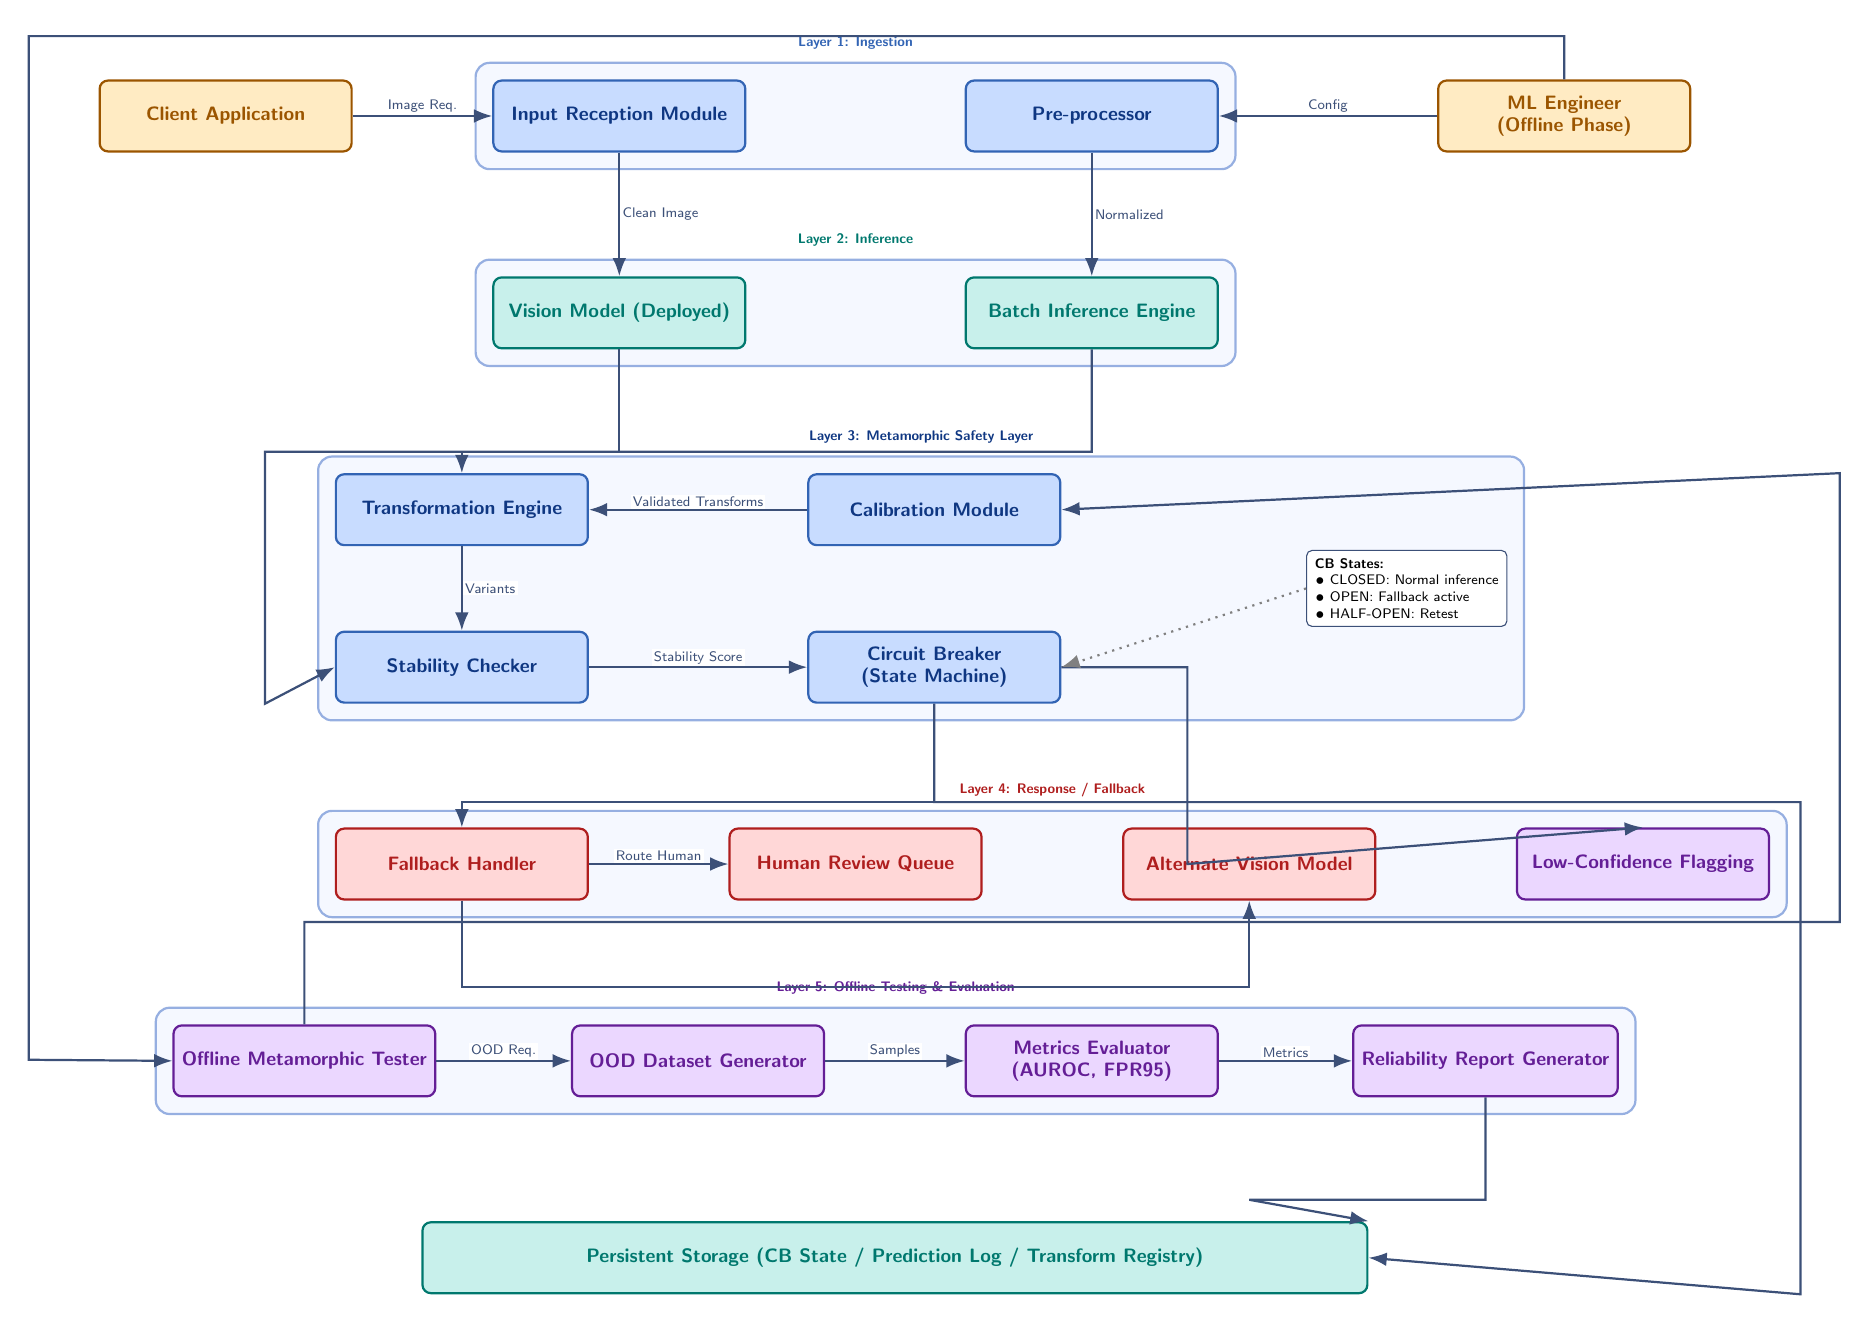
\begin{tikzpicture}[font=\scriptsize\sffamily]
\tikzset{
  CO/.style={draw=steelblue,fill=skyblue,thick,rectangle,minimum width=3.2cm,minimum height=0.9cm,font=\scriptsize\bfseries\sffamily\color{navy},align=center,rounded corners=3pt,inner sep=3pt},
  TC/.style={draw=teal,fill=tealfill,thick,rectangle,minimum width=3.2cm,minimum height=0.9cm,font=\scriptsize\bfseries\sffamily\color{teal},align=center,rounded corners=3pt,inner sep=3pt},
  AC/.style={draw=amber,fill=amberfill,thick,rectangle,minimum width=3.2cm,minimum height=0.9cm,font=\scriptsize\bfseries\sffamily\color{amber},align=center,rounded corners=3pt,inner sep=3pt},
  VC/.style={draw=violet,fill=violetfill,thick,rectangle,minimum width=3.2cm,minimum height=0.9cm,font=\scriptsize\bfseries\sffamily\color{violet},align=center,rounded corners=3pt,inner sep=3pt},
  RC/.style={draw=red2,fill=redfill,thick,rectangle,minimum width=3.2cm,minimum height=0.9cm,font=\scriptsize\bfseries\sffamily\color{red2},align=center,rounded corners=3pt,inner sep=3pt},
  LY/.style={draw=layerbdr,fill=layerbg,thick,rounded corners=5pt,inner sep=6pt},
  FL/.style={->,>=Latex,thick,arrcol},
  RF/.style={->,>=Latex,dashed,thick,red2},
  lb/.style={font=\tiny\sffamily,fill=white,inner sep=0.8pt},
}

\node[AC](client) at (2.0, 5.0){Client Application};
\node[AC](mleng)  at (19.0, 5.0){ML Engineer\\(Offline Phase)};

\node[CO](ingest)  at (7.0, 5.0){Input Reception Module};
\node[CO](preproc) at (13.0, 5.0){Pre-processor};
\begin{pgfonlayer}{background}
  \node[LY,fit=(ingest)(preproc),label={[font=\tiny\bfseries\sffamily\color{steelblue},yshift=1pt]above:Layer 1: Ingestion}](l1){};
\end{pgfonlayer}

\node[TC](vision) at (7.0, 2.5){Vision Model (Deployed)};
\node[TC](batch)  at (13.0, 2.5){Batch Inference Engine};
\begin{pgfonlayer}{background}
  \node[LY,fit=(vision)(batch),label={[font=\tiny\bfseries\sffamily\color{teal},yshift=1pt]above:Layer 2: Inference}](l2){};
\end{pgfonlayer}

\node[CO](te)  at (5.0, 0.0){Transformation Engine};
\node[CO](cal) at (11.0, 0.0){Calibration Module};
\node[CO](sc)  at (5.0,-2.0){Stability Checker};
\node[CO](cb)  at (11.0,-2.0){Circuit Breaker\\(State Machine)};
\node[draw=arrcol,fill=white,rounded corners=2pt,font=\tiny\sffamily,align=left,inner sep=3pt] (cbbox) at (17.0,-1.0){%
  \textbf{CB States:}\\
  $\bullet$ CLOSED: Normal inference\\
  $\bullet$ OPEN: Fallback active\\
  $\bullet$ HALF-OPEN: Retest};
\begin{pgfonlayer}{background}
  \node[LY,fit=(te)(cal)(sc)(cb)(cbbox),label={[font=\tiny\bfseries\sffamily\color{navy},yshift=1pt]above:Layer 3: Metamorphic Safety Layer}](l3){};
\end{pgfonlayer}

\node[RC](fallback) at (5.0,-4.5){Fallback Handler};
\node[RC](human)    at (10.0,-4.5){Human Review Queue};
\node[RC](fbmod)    at (15.0,-4.5){Alternate Vision Model};
\node[VC](lowconf)  at (20.0,-4.5){Low-Confidence Flagging};
\begin{pgfonlayer}{background}
  \node[LY,fit=(fallback)(human)(fbmod)(lowconf),label={[font=\tiny\bfseries\sffamily\color{red2},yshift=1pt]above:Layer 4: Response / Fallback}](l4){};
\end{pgfonlayer}

\node[VC](offtest) at ( 3.0,-7.0){Offline Metamorphic Tester};
\node[VC](oodgen)  at ( 8.0,-7.0){OOD Dataset Generator};
\node[VC](meteval) at (13.0,-7.0){Metrics Evaluator\\(AUROC, FPR95)};
\node[VC](report)  at (18.0,-7.0){Reliability Report Generator};
\begin{pgfonlayer}{background}
  \node[LY,fit=(offtest)(oodgen)(meteval)(report),label={[font=\tiny\bfseries\sffamily\color{violet},yshift=1pt]above:Layer 5: Offline Testing \& Evaluation}](l5){};
\end{pgfonlayer}

\node[TC,minimum width=12.0cm](store) at (10.5,-9.5){Persistent Storage (CB State / Prediction Log / Transform Registry)};

\draw[FL](client.east)--node[lb,above]{Image Req.}(ingest.west);
\draw[FL](mleng.west)--node[lb,above]{Config}(preproc.east);

\draw[FL](ingest.south)--node[lb,right]{Clean Image}(vision.north);
\draw[FL](preproc.south)--node[lb,right]{Normalized}(batch.north);

\draw[FL](vision.south)--++(0,-1.3)--++(-2.0,0)--(te.north);
\draw[FL](batch.south)--++(0,-1.3)--++(-10.5,0)--++(0,-3.2)--(sc.west);

\draw[FL](cal.west)--node[lb,above]{Validated Transforms}(te.east);
\draw[FL](te.south)--node[lb,right]{Variants}(sc.north);
\draw[FL](sc.east)--node[lb,above]{Stability Score}(cb.west);

\draw[FL](cb.south)--++(0,-1.25)--++(-6.0,0)--(fallback.north);
\draw[FL](fallback.east)--node[lb,above]{Route Human}(human.west);
\draw[FL](fallback.south)--++(0,-1.1)--++(10.0,0)--(fbmod.south);

\draw[FL](cb.east)--++(1.6,0)--++(0,-2.5)--(lowconf.north);

\draw[FL](mleng.north)--++(0,0.55)--++(-19.5,0)--++(0,-13.0)--(offtest.west);

\draw[FL](offtest.north)--++(0,1.3)--++(19.5,0)--++(0,5.7)--(cal.east);

\draw[FL](offtest.east)--node[lb,above]{OOD Req.}(oodgen.west);
\draw[FL](oodgen.east)--node[lb,above]{Samples}(meteval.west);
\draw[FL](meteval.east)--node[lb,above]{Metrics}(report.west);

\draw[FL](report.south)--++(0,-1.3)--++(-3.0,0)--(store.north east);

\draw[FL](cb.south)--++(0,-1.25)--++(11.0,0)--++(0,-6.25)--(store.east);

\draw[->,>=Latex,dotted,gray,thick](cbbox.west)--(cb.east);

\end{tikzpicture}%
}
\vspace{0.05cm}
{\tiny\sffamily
\tikz[baseline=-0.5ex]{
  \node[CO,minimum width=2cm,minimum height=0.4cm] at (0,0){Ingestion/Safety};
  \node[TC,minimum width=1.5cm,minimum height=0.4cm] at (3.4,0){Core ML};
  \node[RC,minimum width=2cm,minimum height=0.4cm] at (6.4,0){Response};
  \node[VC,minimum width=2cm,minimum height=0.4cm] at (9.8,0){Offline};
  \node[AC,minimum width=1.5cm,minimum height=0.4cm] at (13.2,0){External};
  \draw[FL](14.9,0)--(16.1,0) node[right]{Normal Flow\,};
  \draw[RF](18.4,0)--(19.6,0) node[right]{Reset/Report Flow};
}}
\end{frame}

\end{document}
